\chapter{Statistics of China's ``South Flood-North Drought'' Pattern and Associated Jet Changes}

%%FIGURE 4.1 Changes in Meiyu and rainfall behavior between 1951-1979 and 1980-2007
\begin{figure}[htbp]
\noindent\includegraphics[width=36pc]{Figures/ch4/changes}
\caption{a) 15-day running mean of the change in rainfall between 1951-1979 and 1980-07, with 95\%/99\% confidence level marked by single/double cross-hatches; b) 15-day running mean of the change in rainband frequency between 1951-1979 and 1980-07, with two-degree smoothing in latitude and confidence levels marked as in a). The significance of rainfall changes is calculated by a permutation method. Time periods are marked as in Figure 1.}
\label{fig:changes}
\end{figure}

%%FIGURE 4.2 Decadal changes in different rainfall types
\begin{figure}[htb]
\noindent\includegraphics[width=36pc]{Figures/ch4/decadal_front}
\caption{1980-2007 versus 1951-1979 changes in frontal and local rainfall for full year (a and b), Pre-Meiyu (c and d) and Post-Meiyu (e and f), with significance at the 95\%/99\% level marked by single/double hatches.}
\label{fig:decadal_front}
\end{figure}

%% FIGURE 4.3 Climatology of rainfall stages including rainfall, jet and most likely rainband configuration, and longitudinal averages.
\begin{figure}
\noindent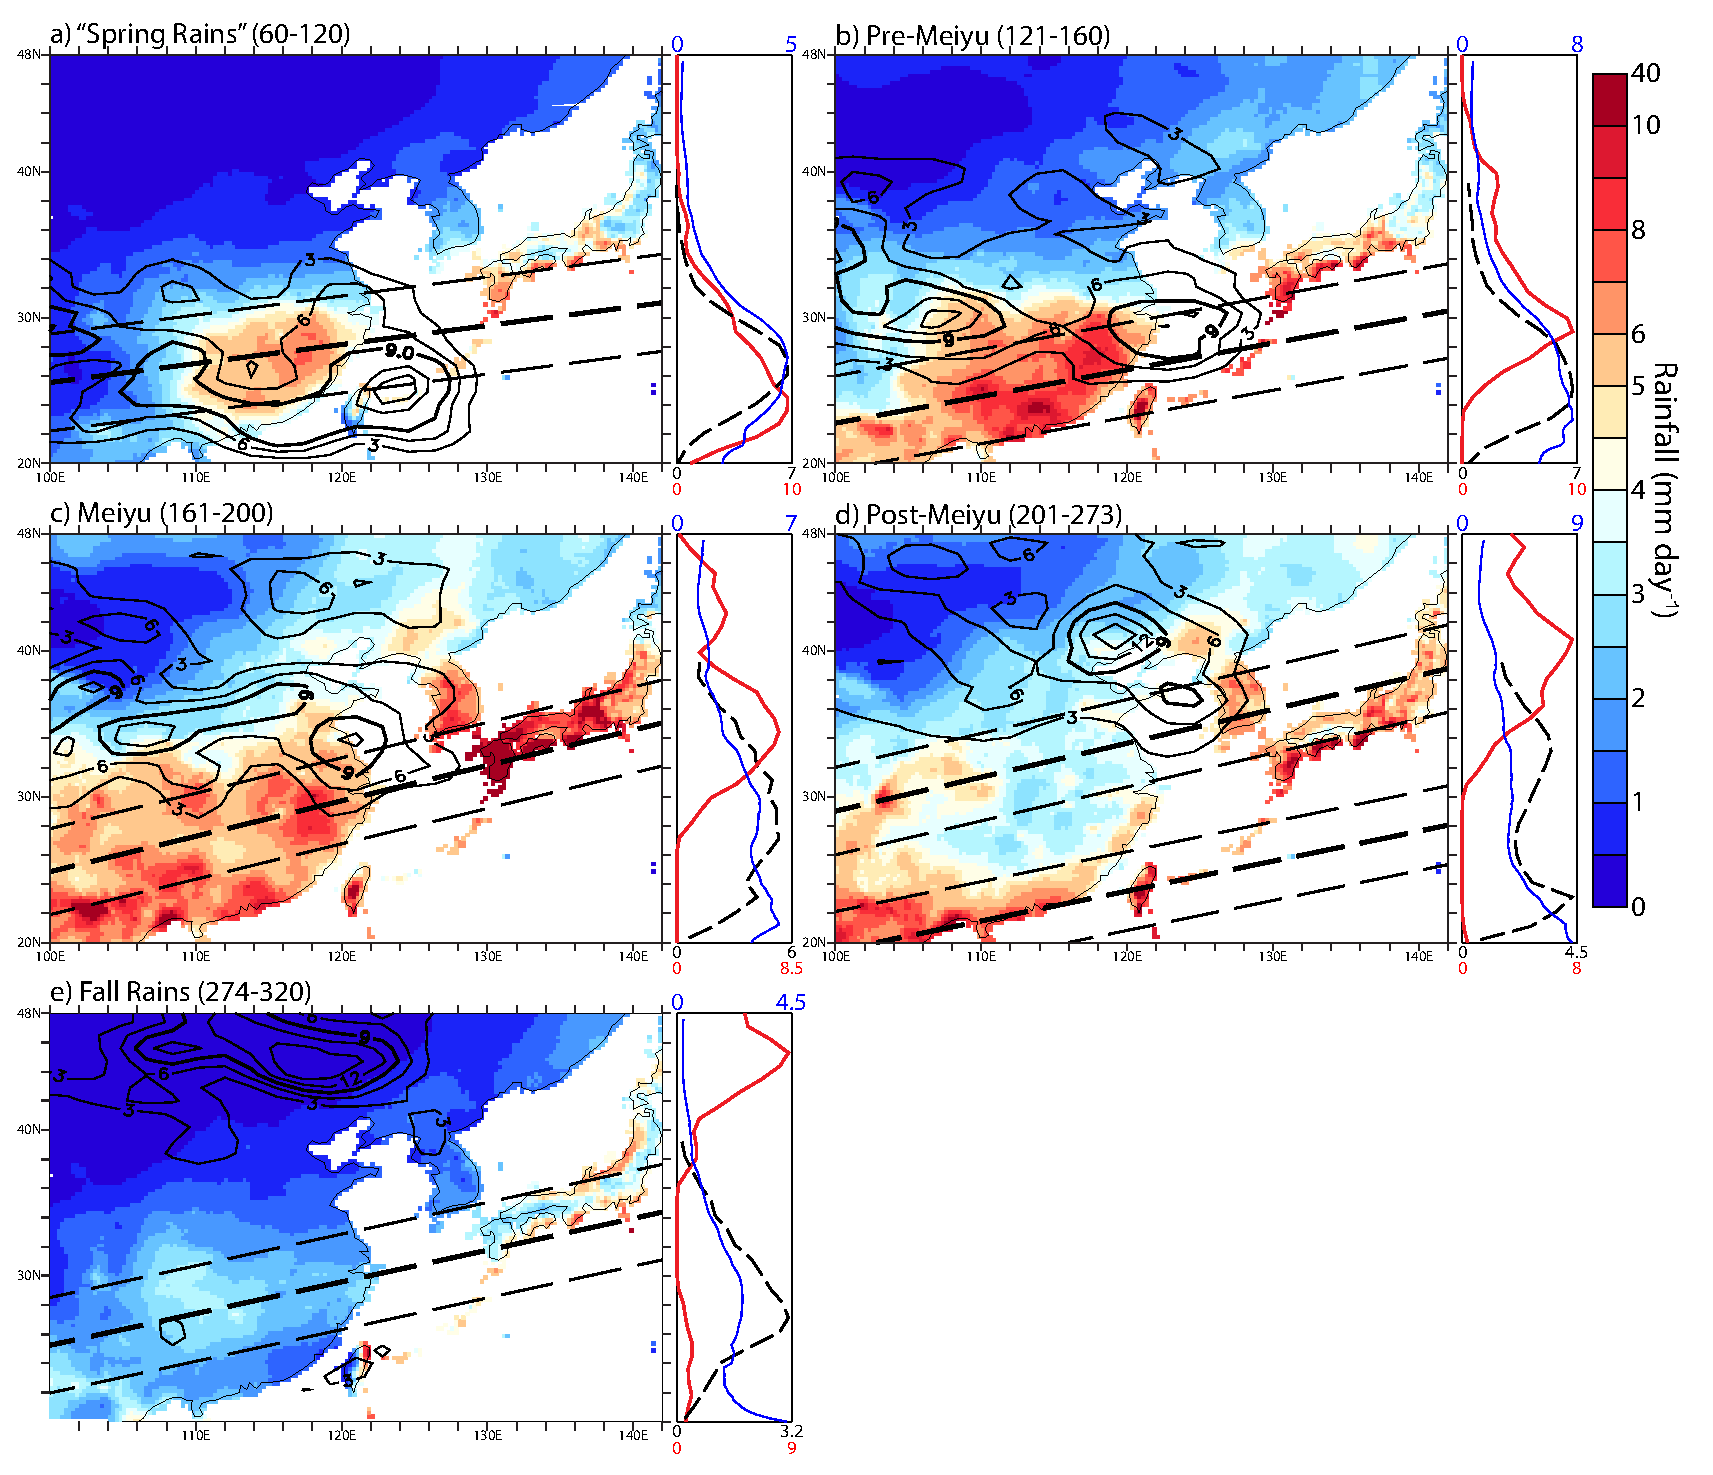
\includegraphics[width=36pc]{Figures/ch4/climo}
\caption{Climatology of East Asian rainfall stages showing rainfall (shading), jet kernel density (contours of probability density in units of $10^{-4}$) and most common rainband position during that stage. Sidebars shows, for each time period, the longitude average over 105-123$^{\circ}$E of rainfall (thin blue line, units of mm day$^{-1}$), jet kernel density (red line, units of $10^{-4}$) and rainband position (dashed black line, absolute probability in \%, 1-degree latitude smoothing). From the Pre-Meiyu to Post-Meiyu, a peak in preferred jet latitude consistently occurs 5 degrees north of a corresponding maximum in rainband frequency.}
\label{fig:climo}
\end{figure}


%% FIGURE 4.4 - 2D spatial distribution of change showing a) full year b) Pre-Meiyu and c) Post-Meiyu
\begin{figure}
\noindent\includegraphics[width=36pc]{Figures/ch4/changes_2d}
\caption{a) Whole year mean rainfall change, showing the South Flood-North Drought pattern; b) Rainfall changes during the Pre-Meiyu (days 121-160) with contours of jet density change overlain; c) Same as c, but for the Post-Meiyu (days 201-273). Statistical significance at 95\%/99\% level overlain with single/double hatches. Sidebars show, for each time period, the longitude average over 105-123$^{\circ}$E of changes in rainfall (thin blue line, units of mm day$^{-1}$), jet kernel density (red line, units of $10^{-4}$) and rainband position (dashed black line, absolute probability in \%, 1-degree latitude smoothing).}
\label{fig:changes_2d}
\end{figure}

%% FIGURE 4.5 - Changes in jet mean between 1951-1979 and 1980-2007 + scatter plots of jet and rainband monthly anomalies.
\begin{figure}[htbp]
\begin{center}
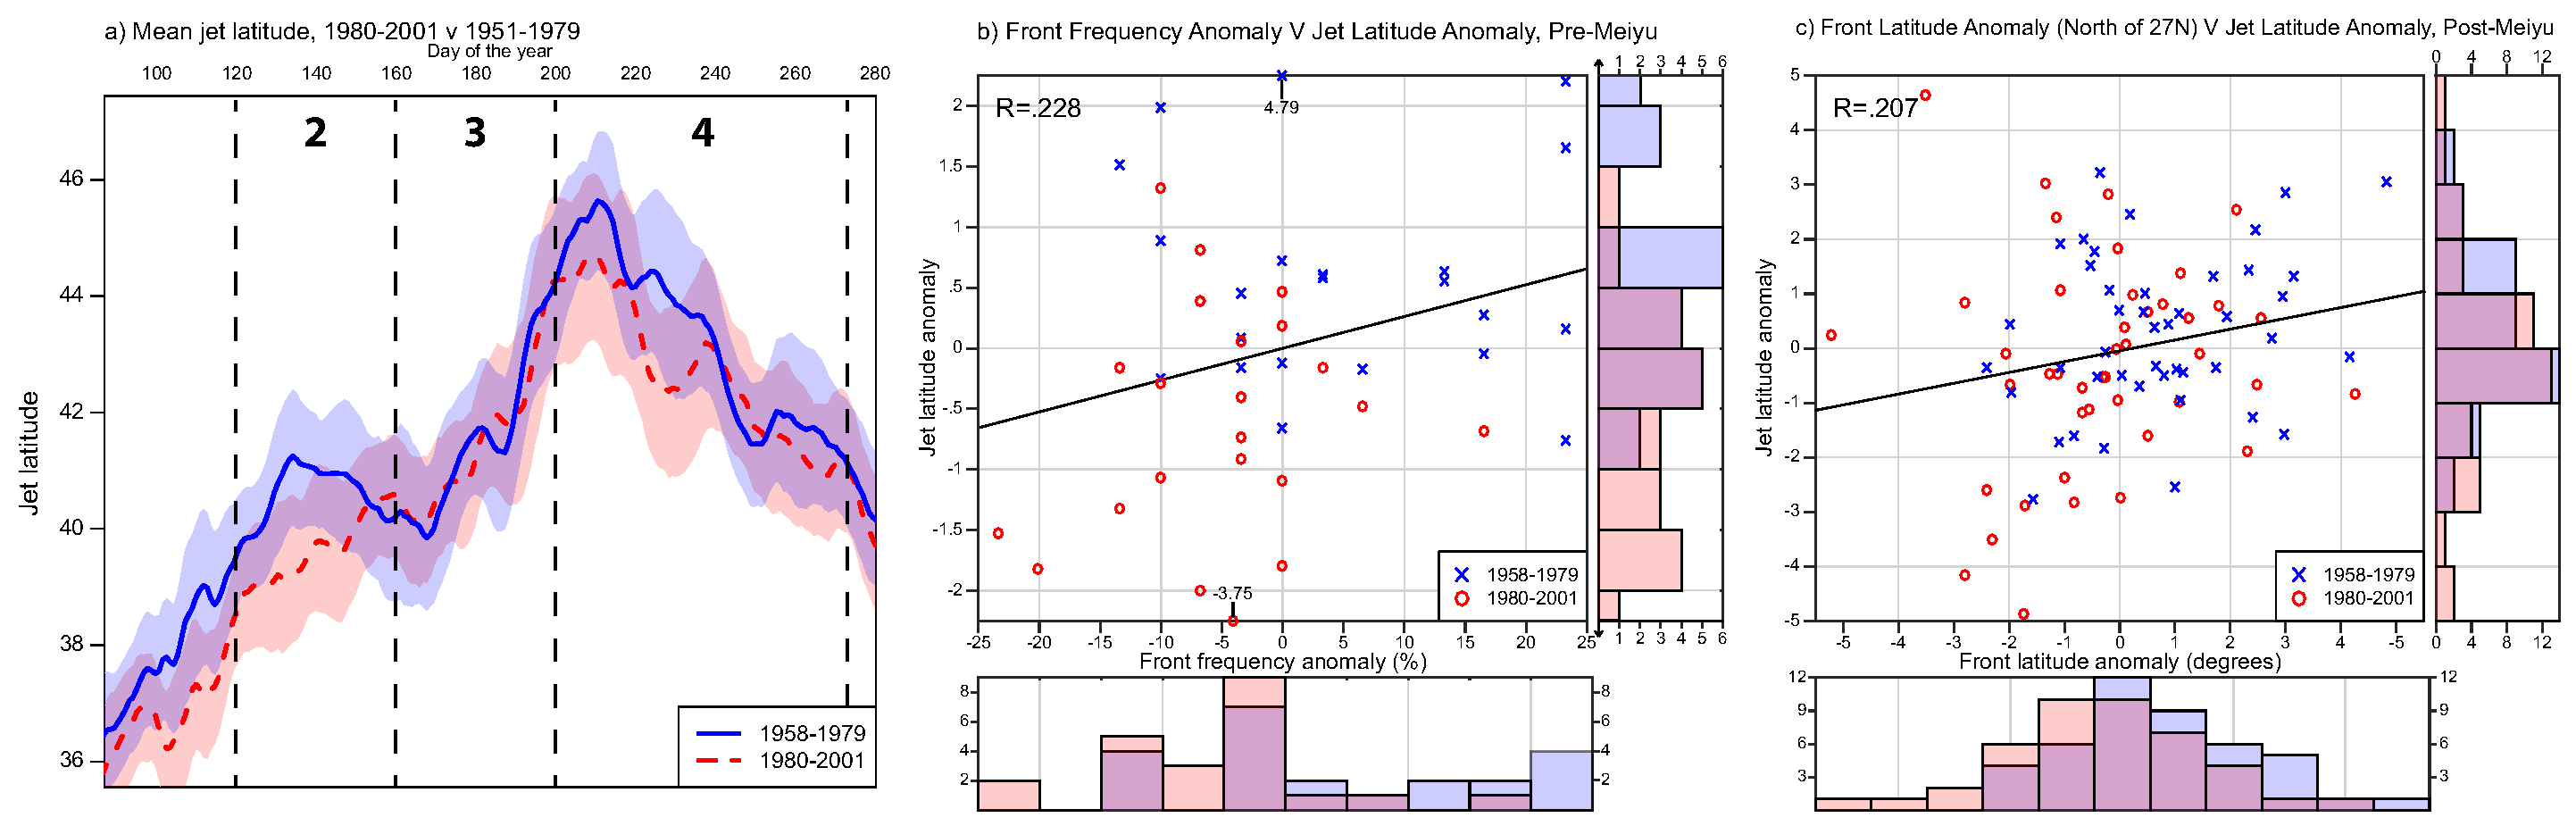
\includegraphics[width=42pc]{Figures/ch4/jet}
\caption{a) 7-day running mean latitude of the westerly jet in the region 90-130$^\circ$E for the years 1958-1979 (blue, solid) and 1980-2001 (red, dashed). Bootstrapped 95\% confidence intervals are shaded. Time periods: 2 - Pre-Meiyu; 3 - Meiyu; 4 - Post-Meiyu; b) Plot of monthly anomalies in rainband frequency versus monthly anomalies in jet latitude during days 121-150 (May) for 1958-1979 (blue X) versus 1980-2001 (red circle); c) Same as b), but showing 30-day anomalies of rainband latitudes during the Post-Meiyu (201-230 and 231-260, each set of 30 days treated as a separate point). Histograms of anomalies are also shown on the side of each figure.}
\label{fig:jet_seasonal}
\end{center}
\end{figure}
